\documentclass[journal ]{new-aiaa}
\usepackage[utf8]{inputenc}
\usepackage{textcomp}
\usepackage{subcaption}
\usepackage{float}

\usepackage{graphicx}
\usepackage{amsmath}
\usepackage[version=4]{mhchem}
\usepackage{siunitx}
\usepackage{longtable,tabularx}
\setlength\LTleft{0pt} 

\title{Optimization of Multiple Rotors}

\author{J. Spencer \footnote{Undergraduate Researcher, Brigham Young University FLOW Lab.}}
\affil{Brigham Young University, Provo, Utah, 84601} 

\begin{document}

\maketitle

\begin{abstract}

This report describes a project completed as part of my research for the Brigham Young University FLOW Lab to discover ideal conditions for airfoil performance. Computational stimulations of propellors allow researchers to perform low-risk studies and develop designs more quickly. The initial rotor in this study was a

This project drew on skills gained throughout the semester to design and execute a code in the julia programming language to find the optimal blade count, blade thickness magnification, and twist angle for a propellor to achieve its maximum efficiency, $\eta$, at a given advance ratio, $J$. This investigation found that thinner rotors are more efficient, especially at negative angles of attack. The implications of these results and possible areas of future research are then discussed.

\end{abstract}


\section*{Nomenclature}

\noindent(Nomenclature entries are identified with their default units.)

{\renewcommand\arraystretch{1.0}
\noindent\begin{longtable*}{@{}l @{\quad=\quad} l@{}}

$J$ & Advance Ratio, \emph{dimensionless} \\
$\alpha$ & Angle of Attack, $rad$ \\
$\phi$ & Angle of Rotation, $rad$ \\
$M_{b}$ & Bending Moment, $N \times m$ \\
$c$ & Chord length, $m$ \\
$D$ & Diameter, $m$ \\
$c_{d}$ & Drag Coefficient, \emph{dimensionless} \\
$\eta$ & Efficiency, \emph{unitless} \\
$\rho$ & Fluid Density, $kg/m^{3}$ \\
$v_{\infty}$ & Freestream Velocity, $m/s$ \\
$c_{l}$ & Lift Coefficient, \emph{dimensionless} \\
$C_{P}$ & Power Coefficient, \emph{dimensionless} \\
$RPM$ & Revolutions Per Minute, $\frac{\emph{rev.}}{\emph{min.}}$ \\
$\sigma$ & Rotor Solidity \emph{dimensionless} \\
$C_{T}$ & Thrust Coefficient, \emph{dimensionless} \\
$C_{Q}$ & Torque Coefficient, \emph{unitless} \\

\end{longtable*}}


\section{Introduction}

\lettrine{P}{ropellors} come in a variety of different shapes and sizes. This paper describes how one propellor, with an APC 10x7 rotor and a NACA 4412 airfoil, was optimized to perform better at a certain advance ratio. The code used for this report could also be applied to different rotors in the future.

This report shows how computer simulations can be used to simulate the performance of propellors without needing to actually create them. It finds that changing the twist angle and the thickness of a propellor does not just shift the curves for its efficiency, thrust coefficient, and torque coefficient; it entirely changes their shape. Propellors with different blade counts also have different curves for these three non-dimensional numbers. All code used for each section of this report can also be accessed through a GitHub repository\footnote{This repository can be accessed in the Rotor-Design branch of \url{https://github.com/JoeSpencer1/497R-Projects}}.


\section{Procedure}

This project was performed using julia programming language.\footnote{julia can be found at \url{https://julialang.org}.} jula is available for free and is useful for a variety of reasons, including that It can store data as vectors and matrices and perform rapid calculations with these objects. It compiles functions in advance, so they can be run more quickly than in some other languages. Function files used for this project, including Xfoil\footnote{Xfoil.jl is available at \url{https://github.com/byuflowlab/Xfoil.jl}}, CCBlade\footnote{CCBlade.jl is available at \url{https://github.com/byuflowlab/CCBlade.jl}}, SNOW\footnote{SNOW.jl is available at \url{https://github.com/byuflowlab/SNOWl.jl}}, and FLOWMath\footnote{FLOWMath.jl is available at \url{https://github.com/byuflowlab/FLOWMath.jl}}, are all designed for julia. These packages provided useful functionality that simplified the design process.

In the rotor design, an airfoil was first created using Xfoil.jl. This airfooil was then attached to a rotor and evaluated using CCBlade.jl. Data about the rotor, including its moments in the normal and tangential directions and its torque, is recorded. This data was then multiplied by a safety factor of $n=1.1$ to determine the maximum allowable loads before the rotor would break or a different material would be required. After constraints were determined, rotor variable types called \emph{rotortest} were created with variable thickness magnification and rotation angle and the program used Optim.jl to find the rotor with the optimal twist angle and thickness magnification for the objective function.

The objective function used in this optimization is listed in equation~\eqref{equation:1}. 

\begin{equation}
	\begin{aligned}
	\label{equation:1}
	f(x_{1}, x_{2}, x_{3}...) = \eta \\
	\end{aligned}
\end{equation}.

In addition to restrictions on the moment and torque mentioned previously, the cord thickness was kept within a factor of two of the original and the twist angle was kept between $-90^{\circ}$ and $90^{\circ}$. These constraints are listed in table~\eqref{tab:2}. They ensured that the optimization found a reasonable solution confined to real limits, shown in table~\eqref{tab:2}.

\begin{center}
\begin{tabular}{l  r}
	 \multicolumn{2}{c}{Table I: Optimization objective, parameters, and constraints}  \\ \hline
  	Maximize: & $\eta$ \\ \hline
  	By varying: & scale of the chord, $c$ \\ 
  	 & twist angle, $\phi$ \\  \hline
  	Subject to & total torque $\leq$ 110\% original \\ 
	 & normal moment $\leq$ 110\% original \\ 
	 & tangential moment $\leq$ 110\% original \\ 
	 & $-90^{\circ} <$ twist angle $< 90^{\circ}$ \\
	 & $50\% <$ chord magnification $< 200\% $ \\ \hline
\end{tabular}
\label{tab:2}
\end{center}

The optimized rotors each had other features in common between them, shown in the last entry of table~\eqref{tab:4}. Ning (page 200) stated that the advance ratio can be found from other variables already listed in the table by equation~\eqref{equation:3}, in which $v_{\infty}$ is the free stream velocity, $n$ is the rotational velocity in revolutions per second, and $D$ is the outer diameter \cite{ComAer}.

\begin{equation}
	\begin{aligned}
	\label{equation:3}
	J = \frac{v_{\infty}}{n D}
	\end{aligned}
\end{equation}

\begin{center}
\begin{tabular}{| c | c | c | c |}
	\multicolumn{4}{c}{Table II: Input value limits in rotor design} \\ \hline
  	 \textbf{Parameter} & \textbf{Default Value} & \textbf{Minimum Value} & \textbf{Maximum Value} \\ \hline
	 Chord Length, & 100\% length & 50\% & 200\% \\ \hline
	 Twist Angle, & $0^{\circ}$ & $-90^{\circ}$ & $90^{\circ}$ \\ \hline \hline
	 Rotational Velocity, $RPM$ & \multicolumn{3}{c|}{6000 RPM} \\ \hline
	 Blade Count & 2 blades & \multicolumn{2}{c|}{1 to 3)}\\ \hline
	 Hub-to-tip ratio & \multicolumn{3}{c|}{10\%} \\ \hline
	 Air Density & \multicolumn{3}{c|}{1.225 kg/$m^{3}$} \\ \hline
	 Diameter & \multicolumn{3}{c|}{0.254 m (10 in.)} \\ \hline
	 Velocity & \multicolumn{3}{c|}{12 m/s (26.84 mph)} \\ \hline
	 Advance Ratio & \multicolumn{3}{c|}{0.472} \\ \hline
\end{tabular}
\label{tab:4}
\end{center}

\section{Optimization}

The objective function, equation~\eqref{equation:1}, was optimized using SNOW.jl. The code was designed so that SNOW.jl found the maximum by finding the minimum of its negative. This is similar to the technique and sign convention described by Martins and Ning in page 10 of Engineering Design Optimization \cite{EngDesOpt}.


\section{Results}

Although the chord thickness changed during the optimization for all blade counts, both the rotor identification and the NACA number stayed the same throughout the optimization. Changing the pitching angle only rotated the rotor blade, and changing the chord length magnified the size of its entire profile uniformly.

\subsection{Results Plot}

Figure~\eqref{fig:5} shows that while the optimized design increased the efficiency of even the rotor with a higher blade count above the rotor pre-optimization, it dramatically decreases the thrust and torque coefficients. The efficiency at higher advance ratios also decreased. These decreases in other rotor properties may not be desired. This illustrates one problem with optimizers: if created correctly, they will do exactly what they are programmed to do and may sacrifice some desirable properties to further optimize the objective function.

\begin{figure}[H]
\centering
 	\subfloat[Efficiency]{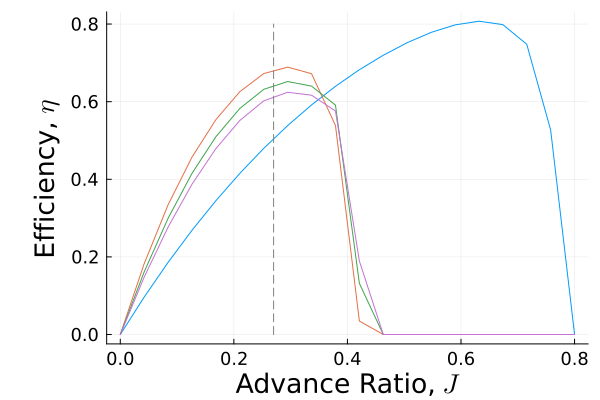
\includegraphics[width = .35\textwidth]{Plots/Figure_1.png}}
	\subfloat[Thrust Coefficient]{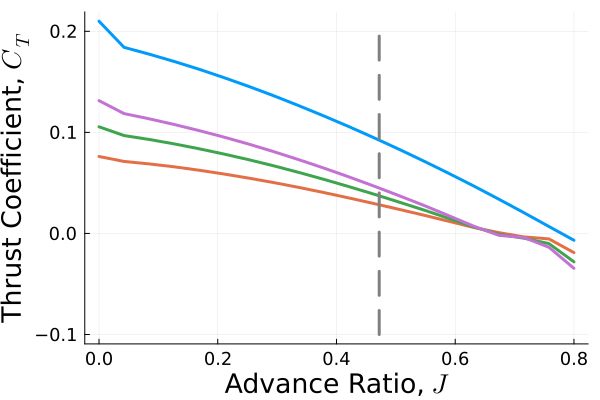
\includegraphics[width = .35\textwidth]{Plots/Figure_2.png}}

	\subfloat[Torque Coefficient]{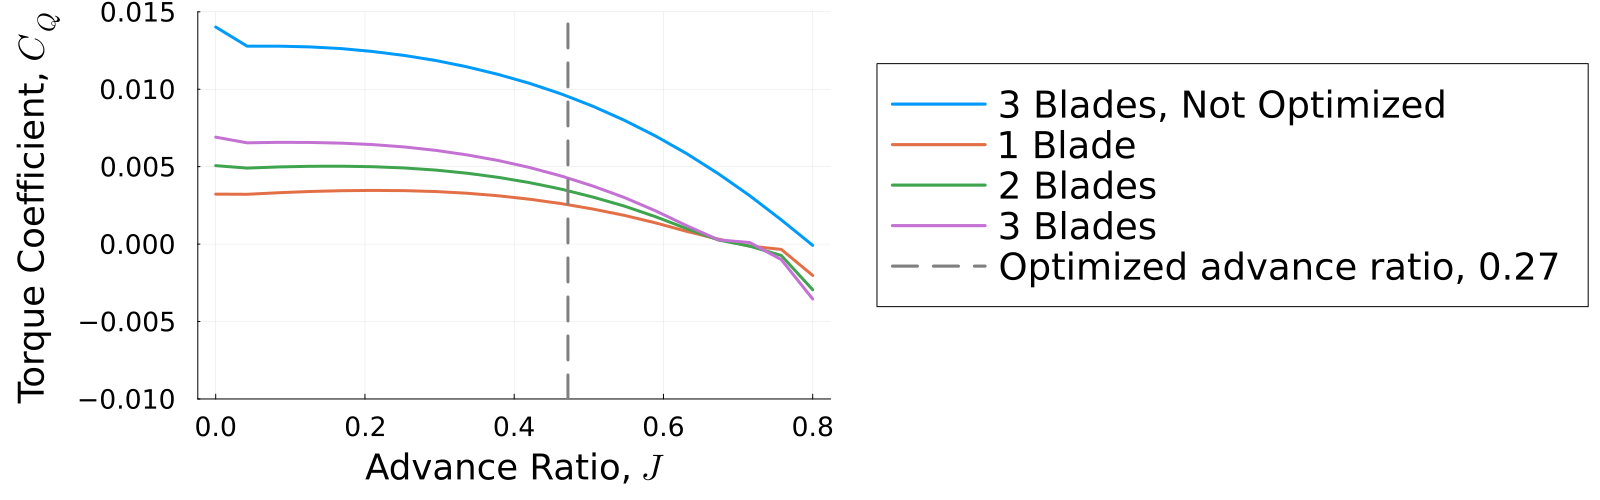
\includegraphics[width = .70\textwidth]{Plots/Figure_3.png}}\hspace{1em}
	\caption{Efficiency, Thrust Coefficients, and Torque Coefficients Compared at Different Advance Ratios}
	\captionsetup{aboveskip=0pt,font=it}
	\label{fig:5}
\end{figure}

If necessary, minimum thrust and torque coefficients could be provided as parameters along with the maximums shown below the objective function in table~\eqref{tab:2}. These could find the angle of rotation and thickness that would provide the maximum efficiency while still maintaining some required thrust. The optimizer might not reduce the rotor to its minimum possible thickness in every case as it did in this optimization.

\subsection{Results Table}

Table~\eqref{tab:6} shows the optimal twist angles and chord magnifications for each different rotor blade count. At the conditions listed in table~\eqref{tab:4}, the optimal chord length magnification was constant, and the optimal angle of rotation was less than $-3^{\circ}$ for each rotor. It gradually became more negative as the blade count increased.

\begin{center}
\begin{tabular}{| c | c | c |}
	 \multicolumn{3}{c}{Table III (Table IV.B): Optimized chord magnification and rotation angles for different blade counts}  \\ \hline
  	 \textbf{Blade Count} & \textbf{Chord Thickness Multiplication} & \textbf{Twist Angle} \\ \hline
  	 3 (Default) & 1.0 & $0^{\circ}$ \\ \hline
  	 2 & 0.50 & $-2.70^{\circ}$ \\ \hline
  	 3 & 0.50 & $-2.88^{\circ}$ \\ \hline
  	 4 & 0.50 & $-2.94^{\circ}$ \\ \hline
\end{tabular}
\label{tab:6}
\end{center}


\section{Discussion}

The propellor was checked at blade counts of 1, 2, and 3. These results found that for all three blade counts, the optimal propellor was as thin as possible, with a small negative angles of attack. The finding about thinner rotor blades being more efficient agreed with Saraf, Nouli, Ravalet, and Bakir's findings, but the negative rotation angle was surprising at first \cite{AxFlFan}.

One lesson learned from this optimization is that the user should be careful what is optimize for, because the computer will optimize exactly what it is told, even if that is not what the user actually wants. An optimization that is written incorrectly or has unseen loopholes can not only give a misleading answer but also waste a lot of time. In the case of this optimization, I think other constraints could have been added to the optimization

\subsection{Efficiency Equation}

One problem with this optimization is that a rotor's efficiency can be found as a function of the advance ratio, the thrust coefficient, and the power coefficient. The equation for efficiency is described by Andrew Ning in \emph{Computational Aerodynamics}, page 200 \cite{ComAer} using the relation below, equation~\eqref{equation:7}.

\begin{equation}
	\begin{aligned}
	\label{equation:7}
	\eta = J \frac{C_{T}}{C_{P}}
	\end{aligned}
\end{equation}

With $J$ kept constant, as it was in this research, this equation can be maximized in either by maximizing $C_{T}$ or by minimizing $C_{P}$, which is equal to $C_{Q}$ multiplied by $2 \pi$. Inspection of figure~\eqref{fig:5} reveals that the optimizer did the latter. The torque coefficient $C_{Q}$ is significantly lower for each rotor. While the thrust coefficient $C_{T}$ did not decrease by as much as $C_{Q}$, it is still much lower than before. Although more efficient, the newly optimized propellor has a much lower solidity and is better suited for a different environment.

\subsection{Angle of Rotation}

The optimal angles of rotation were between $-2.70^{\circ}$ and $-2.94^{\circ}$, as shown in table~\eqref{tab:6}. These negative angles of rotation were surprising at first, because angles near $0^{\circ}$ were expected to be the most efficient. Figure~\eqref{fig:8}, from airfoil analysis conducted earlier in the semester, shows that $0^{\circ}$ angles of attack do not necessarily correspond to the lowest lift and drag coefficients for the NACA 4412 airfoil used in this design. Although that finding was for more simple analysis of an airfoil, it was concluded that a negative angle of rotation was possible.

\begin{figure}[H]
\centering
 	\subfloat[Lift Coefficient]{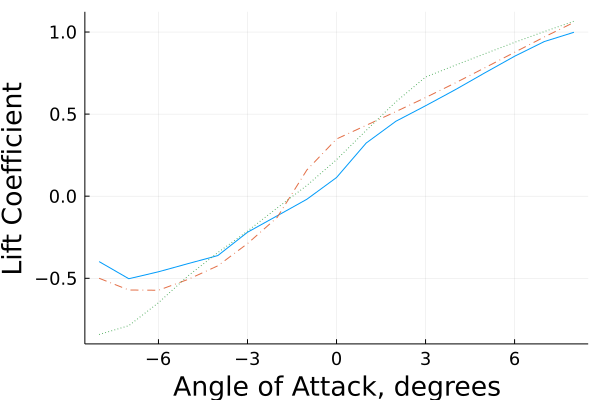
\includegraphics[width = .35\textwidth]{Plots/Figure13.png}}
	\subfloat[Drag Coefficient]{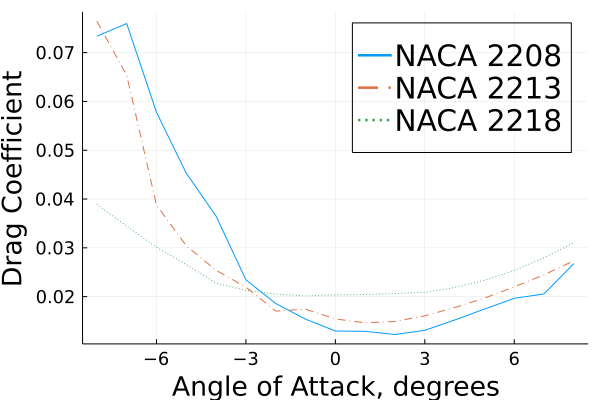
\includegraphics[width = .35\textwidth]{Plots/Figure14.png}}
	\caption{Lift and Drag Experienced by NACA 4412 Airfoils}
	\captionsetup{aboveskip=0pt,font=it}
	\caption*{These plots show how lift and drag change for an airfoil at different angles of attack.}
	\label{fig:8}
\end{figure}


\section{Conclusion}

This optimization combined several different julia packages to find the optimal angle of rotation and rotor chord length for a rotor's efficiency. It found that rotors with very small chord lengths at negative angles of rotation were the most efficient. Other optimizations could be performed by simple editing of the code used in this research to find which rotors perform best in other applications or environments. 


\section{Acknowledgements}

The author would like to thank Adam Cardoza for mentoring him in learning the codes used in the FLOW Lab, directing his research, helping him through questions and challenges that he discovered during his work.



\bibliography{Final_Report}

\end{document}
